\documentclass{beamer}
\usetheme{Madrid}
\usepackage{pgfplots}
\pgfplotsset{compat=1.18, every axis/.append style={grid=major}}
\begin{document}
\begin{frame}{Madrid theme}
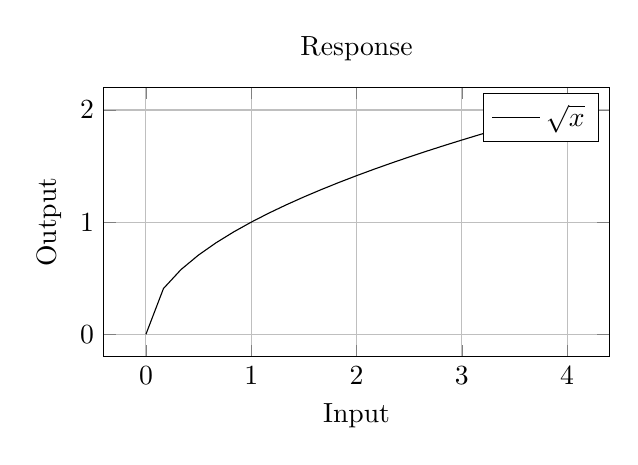
\begin{tikzpicture}
\begin{axis}[width=8cm, height=5cm, xlabel={Input}, ylabel={Output}, title={Response}]
\addplot[domain=0:4, samples=25] {sqrt(x)};
\addlegendentry{$\sqrt{x}$}
\end{axis}
\end{tikzpicture}
\end{frame}
\end{document}
